\chapter{引言}
\label{chap:introduction}

\section{研究背景}
\label{sec:1-research-background}
野火作为陆地生态系统不可或缺的一环，通过干扰与再生机制深刻影响着碳循环及生态演变\cite{pausas2017flammability}。然而，当火势越过荒野、逼近城镇交界地带时，其破坏力便会直接波及人类，其不仅破坏基础设施与周边环境，更严重威胁生命安全。近年来，气候变化与人类活动正在加速重塑野火的行为模式\cite{pausas2021wildfires}。人类对自然生态的干扰及引发的全球变暖，打破了历史固有的火灾周期，这一演变在地中海气候区表现得尤为剧烈\cite{batllori2013climate,moreira2020wildfire}。

从本质上看，自然界的野火绝非孤立事件，而是气候、植被、人类活动等多种驱动因素在不同时空尺度下相互作用的结果\cite{archibald2013defining}。它的爆发既可能源于闪电、火山喷发、落石火花及自燃等自然现象，也常因设备故障等人为意外而起。一旦被点燃，火势的蔓延路径与强度便受制于地形、气象条件以及周围的可燃物。正是由于这种多变量交织带来的高度随机性，野火的准确数学建模至今仍是一个极具挑战性的难题。

早期的研究致力于开发精细的物理机理模型。这类模型从第一性原理出发，以能量守恒与物质消耗的基本定律为基础，将野火视为复杂环境下的多相流体力学与热化学反应过程，如基于计算流体力学的模拟模型\cite{linn2002studying,mell2007physics}。但在实际应用中，纯物理模型面临着两个难以逾越的瓶颈：首先是维度灾难与算力限制，在三维空间中求解大量高度非线性的偏微分方程，消耗的计算资源呈指数级增长，无法满足大尺度、时效性强的灾害预警需求。其次是高维输入数据的获取难度大。微观物理模型对边界条件与初始状态极其敏感，要求输入精确至厘米级的可燃物三维空间结构以及高频的三维风场数据，这类高精度数据几乎不可获取。因此，纯物理模型难以承担实时预警的重任。

既然传统的物理学模型存在瓶颈，不少研究开始探究火险天气与野火活动之间的联系。此类方法存在着一个核心前提：气象条件主导着燃烧的整体走向\cite{abatzoglou2019global,wildfire-review}。基于这一假设，发展出了经验与统计模型。其中最典型的代表是业界极其熟知的火险天气指数（FWI）系统\cite{van1974structure}，以及用于推演中尺度蔓延轨迹的 Rothermel 经验模型\cite{rothermel1972mathematical}。经验统计模型极大降低了对算力与三维高频数据的依赖，并在一定程度上保留了结果的可解释性。然而，此类模型仅依赖气象条件，却忽略了植被与人为因素等其他火灾驱动因素。在预测次日火险时，应综合考量所有火灾驱动要素的时空贡献。

近年来，人工智能领域快速发展。机器学习方法也被得到广泛应用，它能够以数据驱动的方式解析复杂的系统。过去十年间，人工智能驱动的科学研究（AI for Science）范式被应用在地球科学领域。特别是在环境科学与极端气象预测领域，数据驱动模型的应用呈现爆发式增长 \cite{jain2020review}。例如，Pangu-Weather \cite{bi2023pangu} 和 GraphCast \cite{lam2023learning} 等气象大模型，通过利用海量历史数据，在预测精度与时效性上都取得巨大进展，甚至超越了传统数值天气预报（NWP）系统。这充分证明了 AI 在表征复杂物理机制方面的能力。

鉴于野火扩散同样是一个高度非线性、受到气象与地形等多重因素影响的复杂动力学过程，这一问题也备受研究者的关注。针对火灾易发性与风险预测任务，早期的研究采用了决策树（Decision Tree, DT）、随机森林（Random Forest，RF）、支持向量机（Support Vector Machine, SVM）以及多层感知机（Multilayer Perceptron, MLP）等传统机器学习算法 \cite{pourtaghi2016investigation,jain2020review}。如图\ref{fig:ml_wildfire_numbers}所示，各类机器学习方法在火灾领域的应用数量逐年上升。相较于传统统计模型，这些方法在拟合非线性边界时表现出了显著的优势，打破了物理模型算力不够的瓶颈，解决了气象、地形等复杂变量之间的非线性关系。然而，传统 ML 模型通常依赖于繁琐的人工特征工程，且要求将遥感影像或空间图像降维为一维数据进行输入，导致模型难以从全局尺度感知物理规律。因此，要突破这一瓶颈，研究范式向具有强大高维空间表征能力的深度学习（Deep Learning, DL）技术演进。

\begin{figure}[htbp]
    \centering
    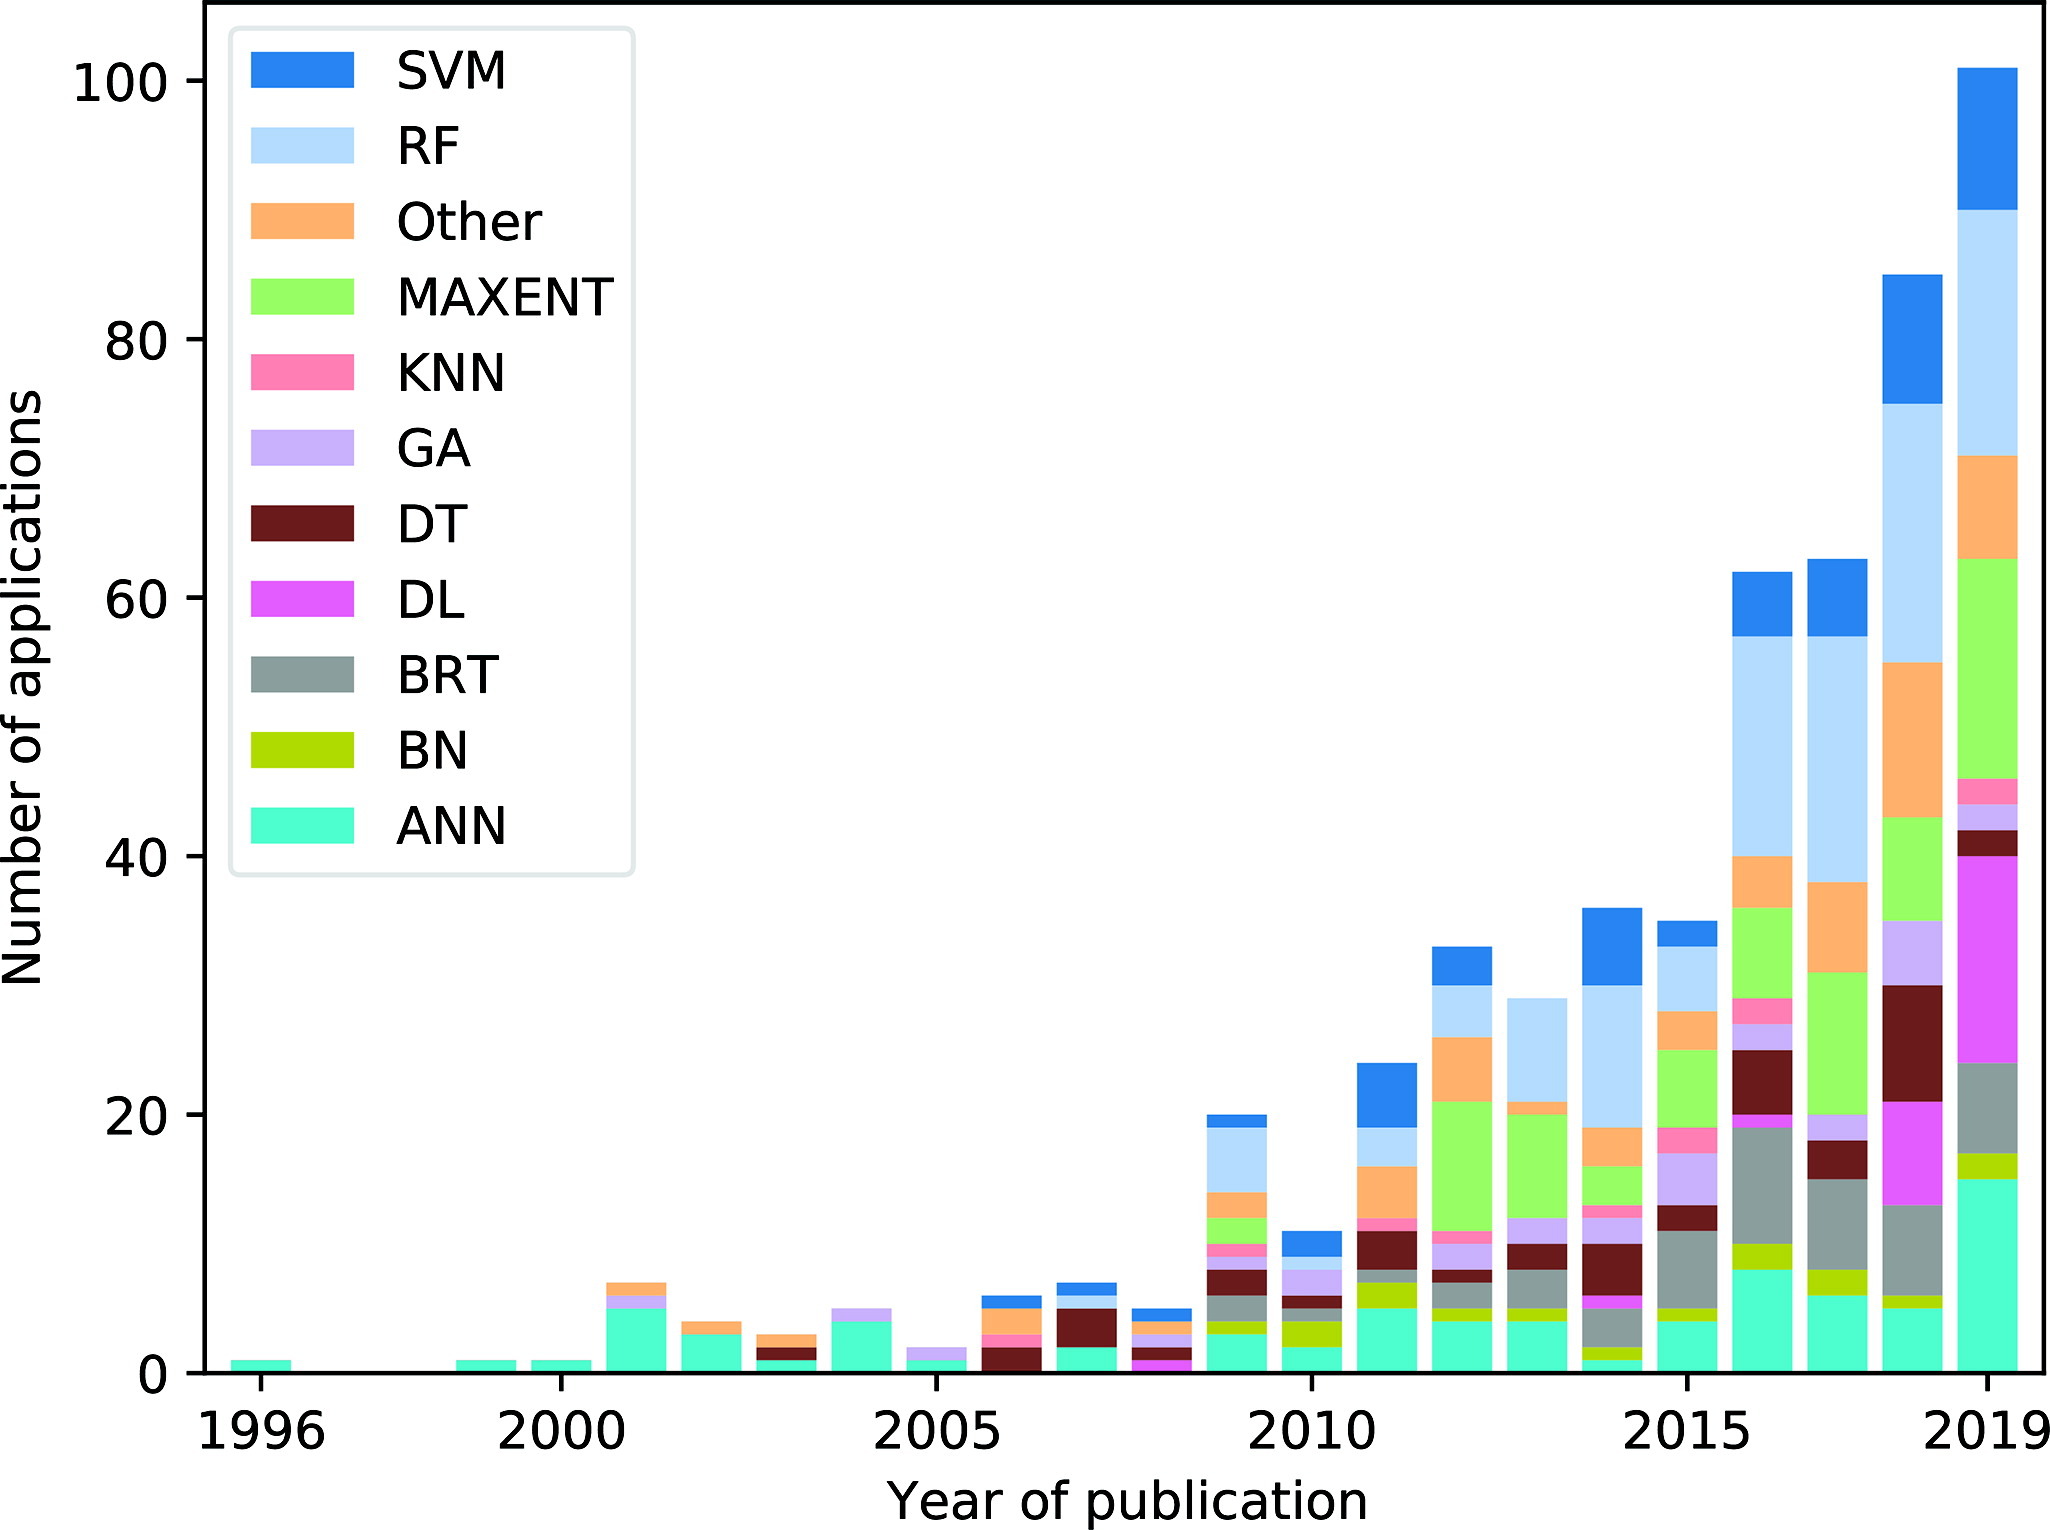
\includegraphics[width=0.6\textwidth]{img/chap1/1-1-ml_wildfire_numbers.jpeg}
    \caption{按类别和年份划分机器学习（ML）应用在野火科学领域的论文数量，引用自\cite{jain2020review}}
    \label{fig:ml_wildfire_numbers}
\end{figure}

随着火灾驱动因素相关数据量的日益增加，特别是卫星遥感技术\cite{forkel2017data}的不断发展，极大地促进了深度学习在野火相关领域的应用。目前，已有诸多研究在野火相关领域中引入了机器学习技术\cite{jain2020review}。

\section{深度学习在野火风险时空预测中的应用}
\label{sec:1-deep-learing}
本节将回顾基于深度学习的野火风险预测模型的最新进展。野火风险预测任务可以被分为三大类：时间序列预测、图像语义分割与分类和时空预测。时间序列模型（如RNN、LSTM、门控循环单元以及Transformer）利用一维特征向量来预测野火风险，而语义分割与分类模型（如CNN和Transformer）则使用二维特征图来生成风险预测。用于时空预测的深度学习模型使用通常将以上两种方法进行结合，输入数据既包含时间序列也包含空间数据。下面我们具体介绍图像语义分割与分类和时空预测任务的进展。

\subsection{图像语义分割与分类}
尽管RNNs和Transformer在捕捉序列间学习任务中的时间依赖性方面表现出色，但这些方法主要对单个像素的时间序列数据进行分类。然而，野火不仅受某个特定小范围的条件影响，还受邻近地区的影响。当RNN使用一维数据输入时，图像的空间结构常常丢失\cite{hu2020spatial}。因此，研究者逐渐转向图像语义分割与分类方法，如卷积神经网络（CNN）、图神经网络（GNN）和Transformer，利用影响因素（如燃料、天气）从$t^{'}<t$开始预测时间$t$的野火风险。这些方法依赖于二维图像输入，能够利用野火传播的空间特性。

作为深度学习领域的基础网络，卷积神经网络（Convolutional Neural Network，CNN）通过卷积操作提取局部空间特征，非常适合捕捉野火风险预测所需的空间信息。例如，\textcite{zhang2019forest}采用了修改版的 AlexNet\cite{krizhevsky2012imagenet}，利用中国云南省的年度火点地图和春季平均影响因素，将图像划分为野火易发区域，模型能够在最后一层的卷积神经网络中通过 softmax 映射输出野火风险概率图。在作者的实验中，发现CNN实现了最高的整体准确率，并利用信息增益率方法，分析了各种野火驱动因素的贡献，确定温度、风速和降水量是最具影响力的因素。在此基础上，生成了全球季度野火易感性地图\cite{zhang2021deep}。一些研究采用了更深层的或结构优化的CNN网络。例如，\textcite{oak2024novel}利用VGG16预测加拿大魁北克的野火易感性，\textcite{nur2022creation}应用了一种元启发式优化算法，对美国普卢马斯国家森林中CNN模型的野火易感性图谱进行微调。此外，一些工作开发混合架构或端到端模型处理数据，预测野火蔓延\cite{allaire2021emulation,li2023predicting}。

除了卷积神经网络（CNN），图神经网络（GNN）和 Transformer 等其他图像分割方法也被应用于野火风险预测。与 CNN 相比，GNN 更擅长处理非欧几里得结构的数据\cite{jiang2022modeling}，而 Transformer 的多头自注意力机制在对图像内的长距离语义依赖进行建模时更为有效。

\subsection{时空预测}
\label{sec:1-2-spatiotemporal-prediction}
上述提到的时间序列预测方法和图像分割与分类方法，分别在捕捉时间依赖性和空间依赖性方面各具优势。然而，它们无法同时处理空间与时间数据，也难以捕捉复杂的跨时空交互模式\cite{prapas2021deep}。为了整合空间结构与时间序列数据，许多研究将两者结合，也将野火预测任务转化成时空序列预测任务。本文的任务即属于时空预测，图\ref{fig:1-2-time-space}展示了野火时空预测任务示意图。实现这种结合主要有三种方法：分离式时空建模（separated spatial and temporal modeling）、耦合式时空建模（coupled spatiotemporal modeling），以及空间增强型耦合时空建模（spatially enhanced coupled spatiotemporal modeling）\cite{xu2025deep}。

\begin{figure}[htbp]
    \centering
    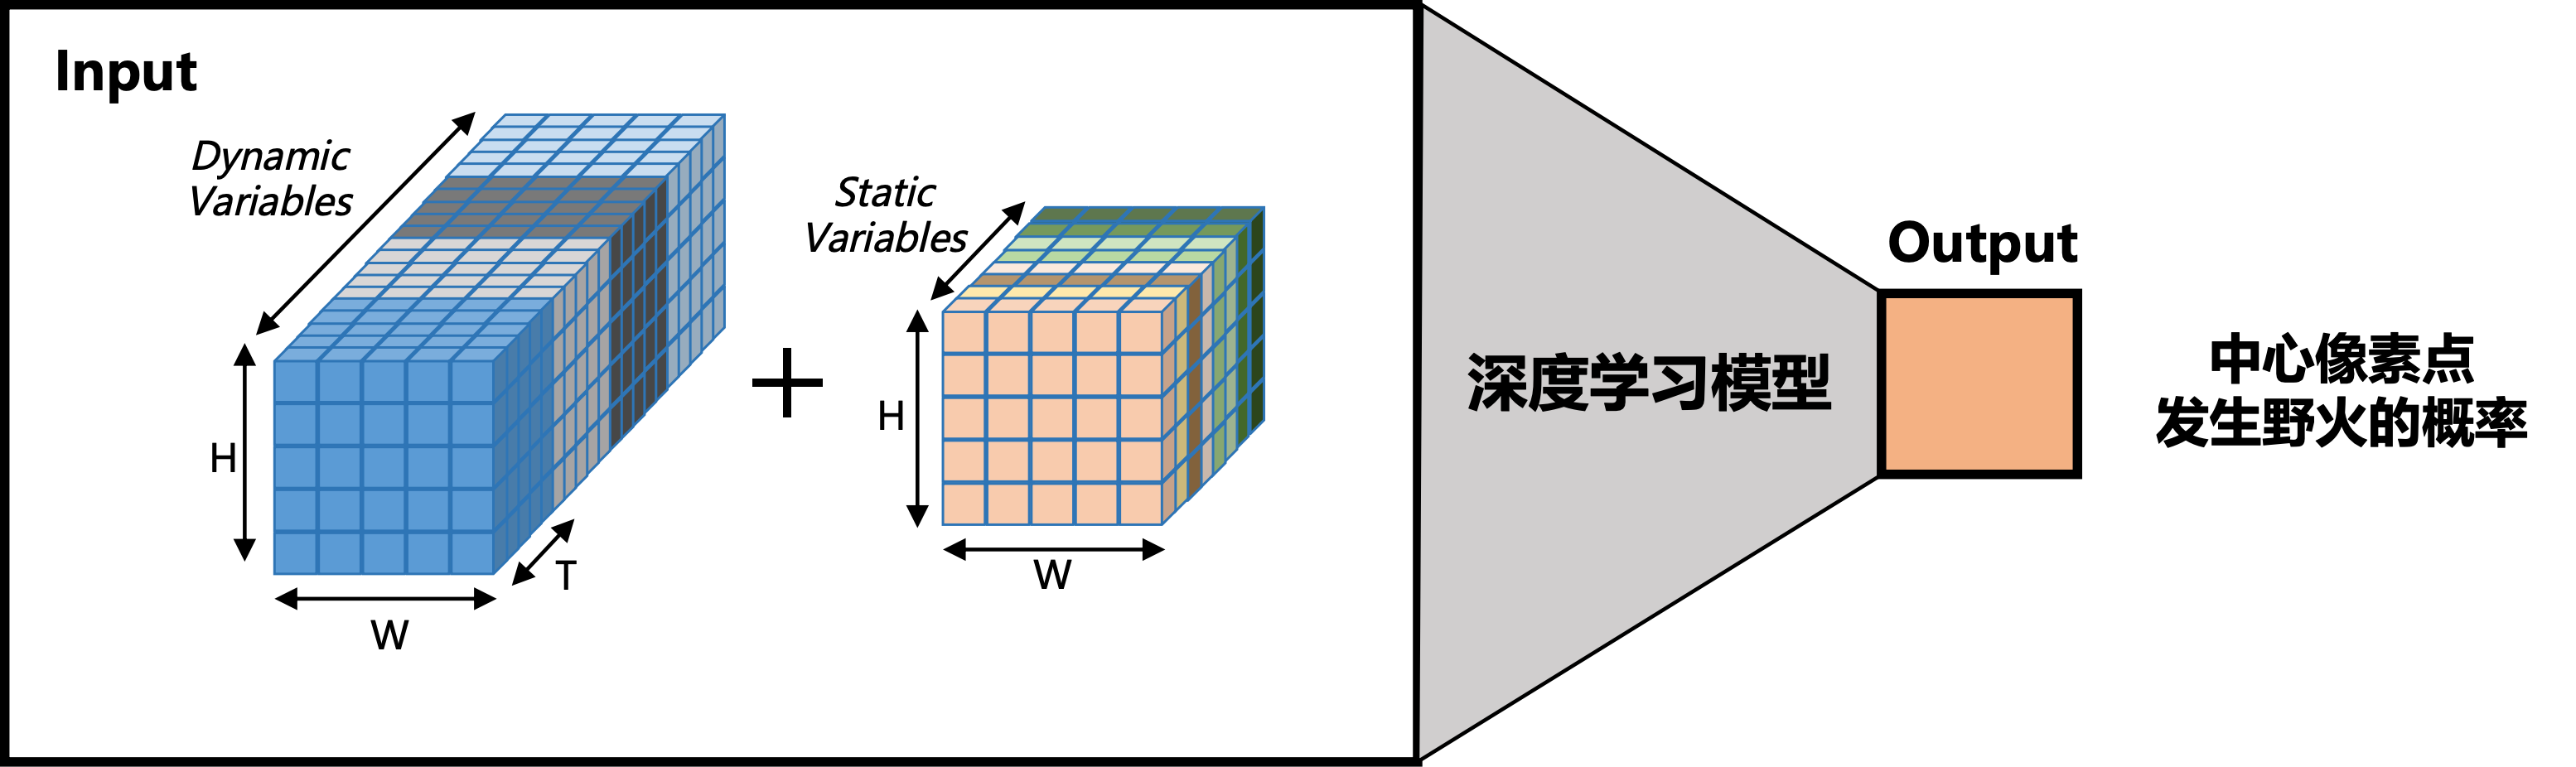
\includegraphics[width=0.9\textwidth]{img/chap1/1-2-time-space.png}
    \caption{野火时空预测任务示意图}
    \label{fig:1-2-time-space}
\end{figure}

具体而言，分离式时空建模是指利用空间建模方法将空间特征抽象为一维特征向量，随后将其输入到时间预测模型中。耦合式时空建模则是将 RNN 中的一维张量转换为三维张量，融入了空间维度，并使用卷积或图结构（而非权重矩阵乘法），基于相邻网格单元当前与过去的状态来决定该网格单元未来的状态。空间增强型耦合时空建模是在正式进入时空建模阶段之前，先引入 CNN 或基于图的方法来提取空间特征\cite{xu2025deep}。

分离式时空建模方法将空间与时间特征的提取分步进行。如图\ref{fig:1-2-separated-modeling}所示，首先在每个时间步上使用卷积神经网络（CNN）等模块对多维空间数据进行特征提取，随后将提取到的二维空间特征降维成一维的全局表征，然后将这些一维向量输入到时间序列模型（如 LSTM 或 GRU）中，以捕捉火灾随时间演变的动态规律，最后通过分类器（或反卷积层映射）输出最终的火灾风险概率。这种范式有效利用了 CNN 在识别复杂空间模式方面的强大能力，又发挥了LSTM或GRU在时间序列建模上的独特优势，从而较好地捕捉野火系统中的时空动态变化\cite{huot2020deep,zhang2022dynamic,marjani2024cnn}。

\begin{figure}[htbp]
    \centering
    \begin{minipage}{0.48\textwidth}
        \centering
        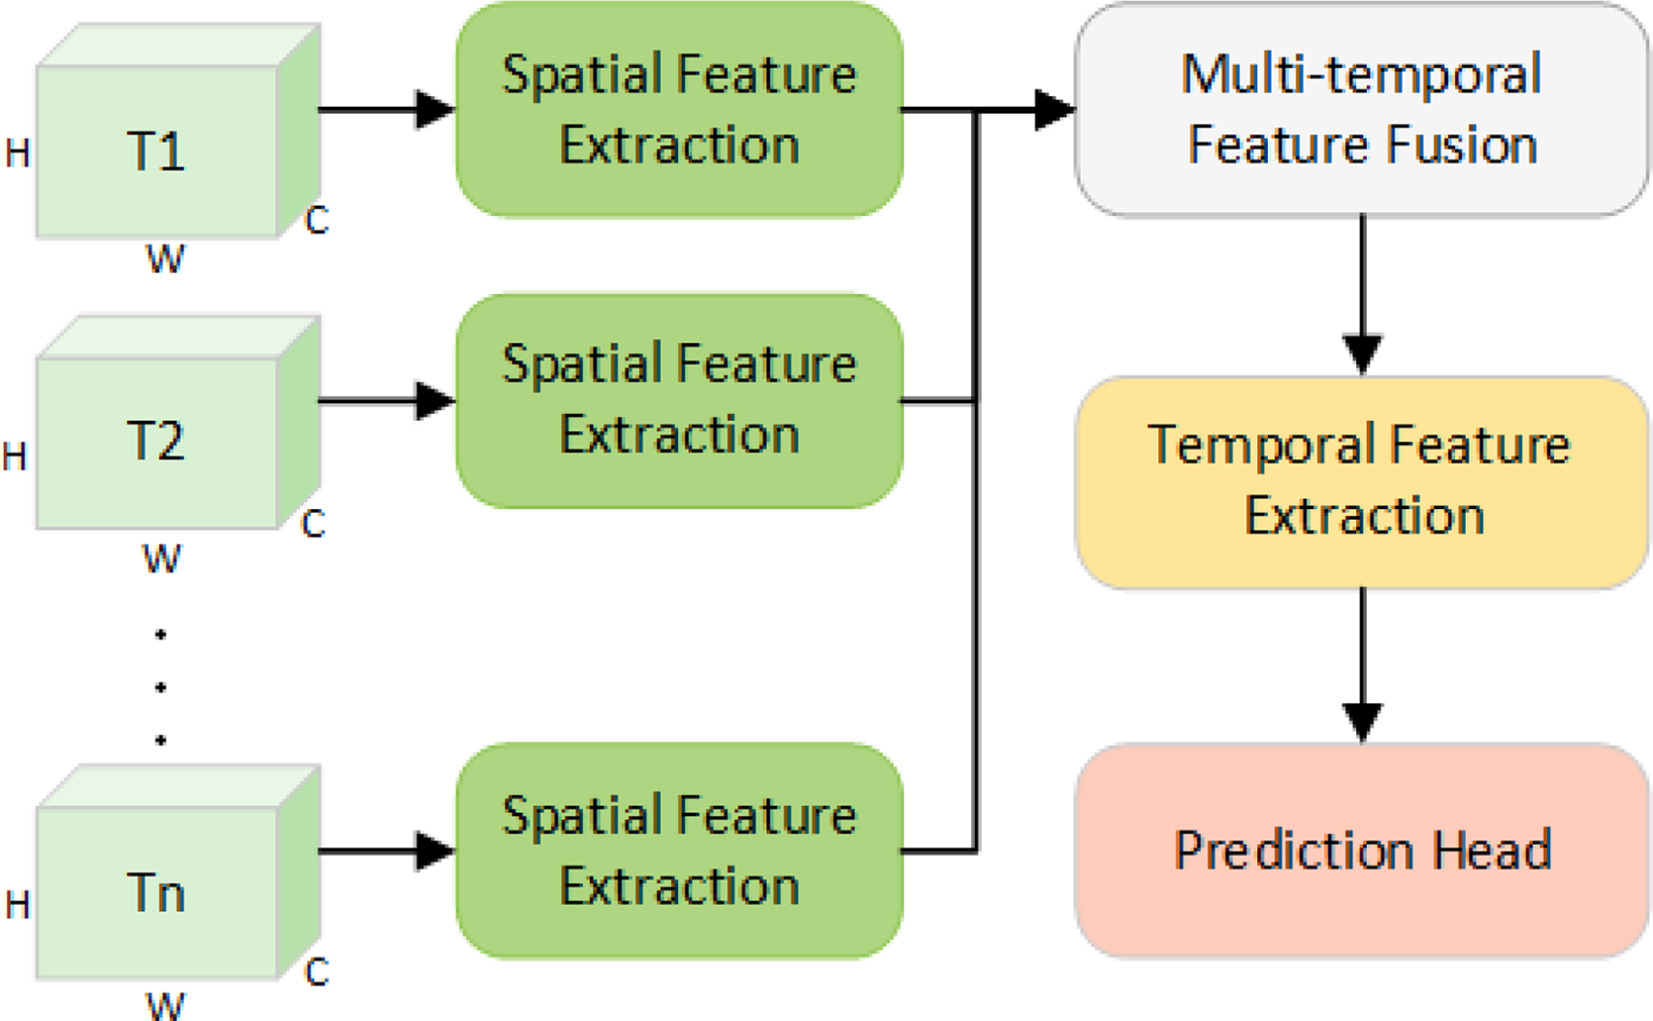
\includegraphics[width=\textwidth]{img/chap1/1-2-separated-modeling.jpg}
        \caption{分离式时空建模示意图，引用自\protect\cite{xu2025deep}}
        \label{fig:1-2-separated-modeling}
    \end{minipage}
    \hfill 
    \begin{minipage}{0.48\textwidth}
        \centering
        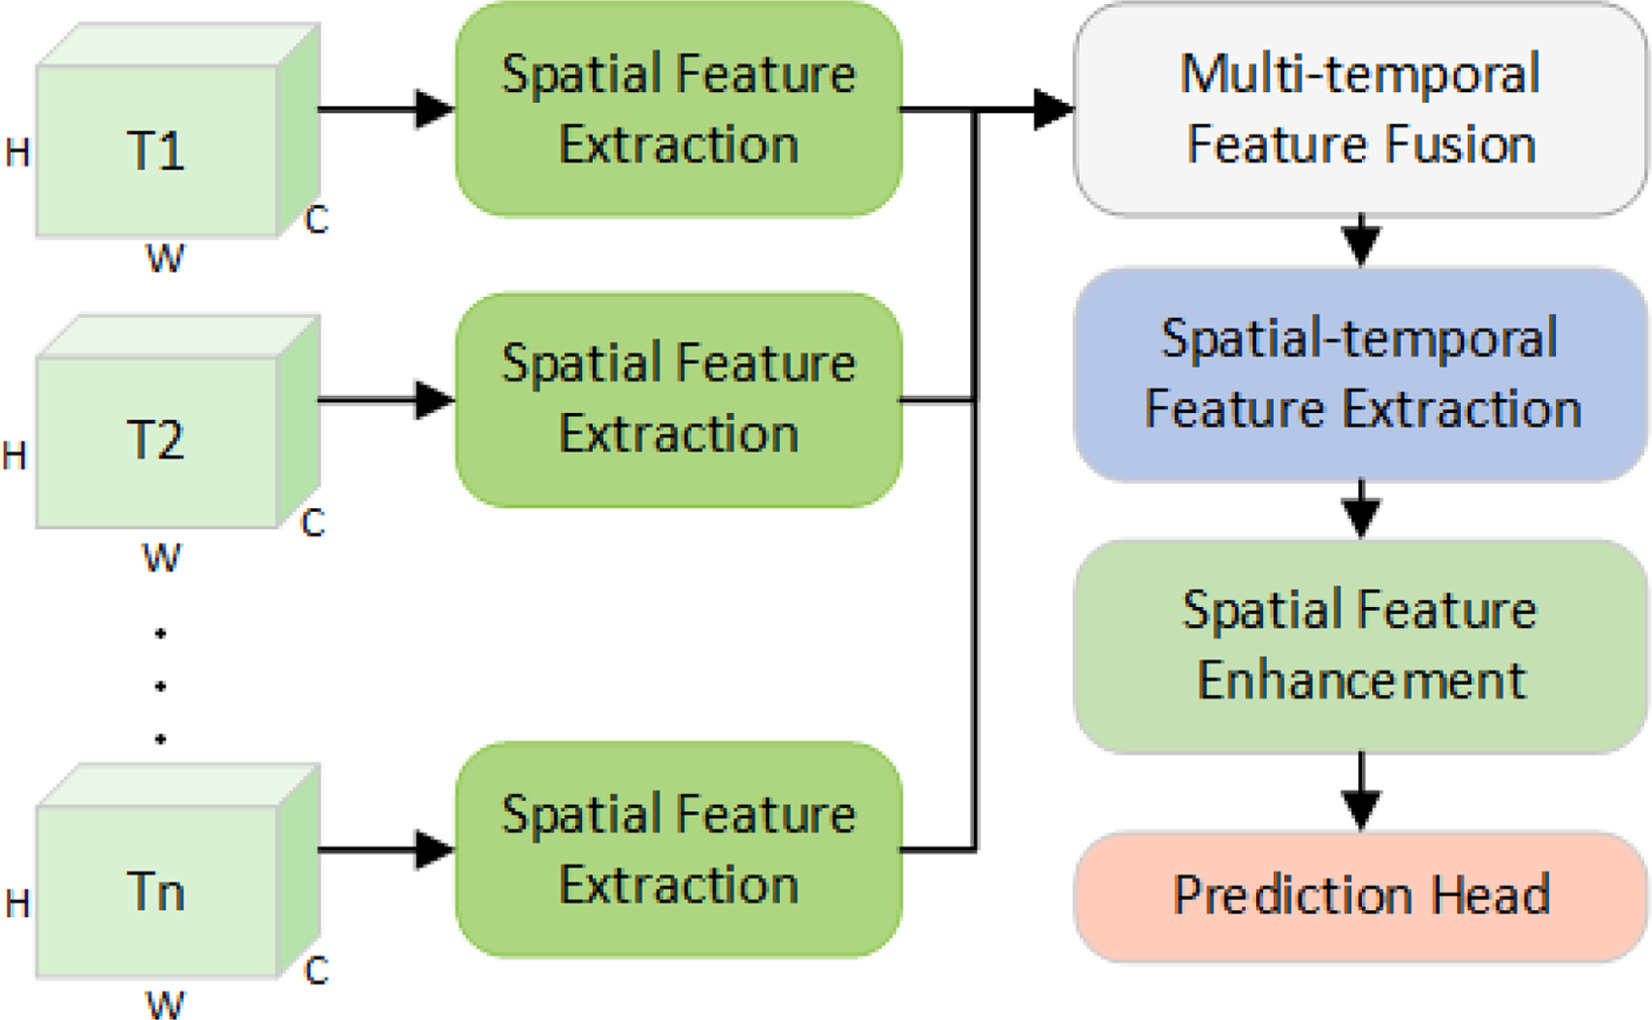
\includegraphics[width=\textwidth]{img/chap1/1-2-spatially-enhanced.jpg}
        \caption{一个典型的空间特征增强型耦合时空野火风险预测模型图，引用自\protect\cite{xu2025deep}}
        \label{fig:1-2-spatially-enhanced}
    \end{minipage}
\end{figure}

视线转向耦合式时空建模，卷积长短期神经网络（ConvLSTM）无疑是被广泛采用的框架。以 \textcite{burge2020convolutional} 的工作为参照，该团队将三组在地形、风场、湿度及植被密度上具有截然不同分布的模拟数据集进行拼合，旨在校验 ConvLSTM 捕捉火情蔓延动态的理论上限。实测反馈极为清晰：该架构的预测准确率直接超越了 CNN 的基准。\textcite{prapas2021deep} 则把研究靶点设在希腊全境的次日火险预警上，他们比较了随机森林模型（RF）、时间序列预测算法（LSTM）、图像分类方法（CNN）以及时空建模方法（ConvLSTM），并得出了几个关键发现。对于 RF 模型，训练数据的构建方式是计算每个空间位置在预测日期前 10 天各个驱动因素的平均值，从而生成维度为 $f\times 1$ 的数据集（其中 $f$ 为驱动因素的数量）。LSTM 模型采用时间序列输入，数据维度为$f\times t$，其中 $t$ 代表时间序列的长度（10天）。对于图像分类任务，空间数据被构建为以目标点为中心的空间图块（patches），其维度为$f\times h\times t$（其中 $h$ 和 $w$ 分别为图像的高度和宽度）。最后，对于使用 ConvLSTM 的时空预测任务，数据集的维度为 $f\times h\times w\times t$。结果表明，LSTM 和 ConvLSTM 的表现优于 RF 和 CNN。在评估二分类结果时，LSTM 总体上优于 ConvLSTM。

空间增强型耦合时空建模在耦合时空建模的基础上，将卷积层与 ConvLSTM 结合，以进一步强化空间特征的提取。如\ref{fig:1-2-spatially-enhanced}所示，在将数据送入时间模型（如 ConvLSTM）之前，会先进行降维处理。与分离式时空建模方法相比，这种方法在整个建模过程中往往能保留一定程度的空间信息，从而在最终的预测结果中，能够保留更精细的空间模式\cite{xu2025deep,ji2024global,he2024deep}。

本节回顾了应用于野火风险预测的深度学习方法的最新进展，重点关注其从时间、空间建模向时空序列建模的演进。得益于其优秀的架构，深度学习模型在捕捉非线性关系方面表现出色，能够对高维时空数据中复杂的关系进行建模，包括气象变量、植被指数、地形特征和社会因素等，从而更好地实现对野火风险的预测。

\section{本论文主要内容及结构}
\label{sec:denotation}
本论文除附录外共分为六个章节。第一章为引言，阐述研究背景与意义，并综述深度学习模型在野火风险预测领域的应用。第二章详细介绍FireCube数据集，包括区域概况及时空数据构建，采样方式及训练数据，特征变量分析。第三章阐述基于Swin Transformer的架构设计，包括气象动力学特征提取模块，静态地貌特征编码模块，特征融合模块以及物理信息启发的数据重构与注意力偏置。第四章展示实验结果与评估，包括模型训练，实验设置与性能对比，消融实验等。第五章为可解释性分析部分，重点阐述基于SHAP的归因分析和交叉注意力融合机制分析。第六章为总结与讨论，对本研究进行总结，并指出局限性和未来展望。附录详细介绍了研究中使用的算法等。
